%!TEX encoding = UTF-8 Unicode
\documentclass{article}[encoding=U]
\usepackage{listings}
\usepackage{xcolor}
\usepackage{titling}
\usepackage{graphicx}
\usepackage[bottom]{footmisc}
\usepackage{hyperref}
\usepackage{multicol}


\newcommand{\logo}[1]{%
	\postauthor{%
	\end{tabular}\par\end{center}
	\begin{center}\includegraphics[scale=0.8]{#1}\end{center}
\vskip0.5em}%
}

%%%%%%%%%%%%%%%%%%%%%%%%%%%%%%%%%%%%
%   CONFIGURAZIONI
%%%%%%%%%%%%%%%%%%%%%%%%%%%%%%%%%%%%
\title{
	TURING \\
	\large disTribUted collaboRative edItiNG \\
	\large Reti di Calcolatori - Laboratorio}
\author{
	Federico Gerardi \\
	Matricola: 508082 \\
	\texttt{federicogerardi94@gmail.com}}
\logo{assets/logo}

\lstset{
	basicstyle=\footnotesize,
	aboveskip=0.5cm,
	belowskip=0.5cm,
	showstringspaces=false,
	keywordstyle=\bfseries,
	numbers=none,
	breaklines=true,
	rangeprefix = \#,
	includerangemarker = false,
	frame=single
}
\lstdefinelanguage{JSON}{%
	keywords={true, false, null, undefined},
	keywordstyle=\bfseries,
	ndkeywordstyle=\bfseries,
	sensitive=false,
	comment=[l]{//},
	morecomment=[s]{/*}{*/},
	commentstyle=\ttfamily,
	stringstyle=\color{blue}\ttfamily,
	morestring=[b]',
	morestring=[b]`,
	morestring=[b]"
}
\definecolor{lightgray}{gray}{0.95}

\begin{document}
\maketitle
\bigskip
\begin{abstract}
TURING - \textit{disTribUted collaboRative edItiNG} è una piattaforma client-server realizzata come progetto finale per il modulo di Laboratorio dell'esame di Reti di Calcolatori della Laurea Triennale in informatica dell'Università di Pisa. Il progetto si basa sulla creazione di un sistema di document editing multiutente distribuito (simile a quello offerto da Docs di Google), che gestisce permessi di modifica e operazioni di aggiornamento dei contenuti dei documenti esistenti in maniera concorrente e consistente. Questo paper fornirà una panoramica della sua infrastruttura e illustrerà alcune scelte implementative.
\end{abstract}

\newpage

\tableofcontents
\clearpage

\section{Funzioni della piattaforma}
Le funzionalità che la piattaforma implementa sono le seguenti:
\begin{itemize}
	\item Creazione di un nuovo utente;
	\item Login dell'utente all'interno della piattaforma;
	\item Inizio della fase di modifica di una specifica sezione di un documento;
	\item Terminazione della fase di modifica e aggiornamento della relativa sezione sul server;
	\item Visualizzazione di una sezione del documento;
	\item Visualizzazione di un intero documento
	\item Operazioni per l'invio/ricezione di messaggi in chat condivisa tra gli editor di più sezioni appartenenti allo stesso documento.
	\item Condivisione dei permessi di accesso ad un documento di cui si è i proprietari ad altri utenti;
	\item Gestione delle notifiche generate in seguito alla ricezione dei permessi di accesso ad un documento.
\end{itemize}

\section{Esecuzione dell'Applicazione}
\subsection{Compilazione}
La compilazione viene gestita attraverso il toolkit \textit{Maven}, che ci permette di definire delle apposite routine\footnote{È definita anche una routine per \textit{pulire}} che si occuperanno di effettuare il packing sia del client che del server di TURING.\\


\subsection{Server}
\subsection{Client}

\section{Interfaccia utente}
\subsection{Argomenti a Linea di Comando}
Utilizzando alcuni argomenti da linea di comando, è possibile specificare alcune preferenze\footnote{È possibile avere la lista completa attraverso l'invocazione dei due programmi con il flag \textit{-h} o \textit{--help} } del comportamento sia del client che del server. \\
In particolare, le seguenti sono i parametri di connessione personalizzabili attraverso gli argomenti a riga di comando:

\begin{itemize}
	\item\textit{--tcp-command-port}: Numero di porta utilizzato per la connessione relativa allo scambio di comando/responso;
	\item\textit{--udp-multicast-port}: Numero di porta utilizzato\footnote{Opzione disponibile unicamente sul client} per lo scambio di messaggi multicast;
	\item\textit{--rmi-port}: Numero di porta utilizzato per la connessione TCP sfruttata per effettuare chiamate RMI\footnote{L'unica funzione che sfrutta RMI è la registrazione di nuovi utenti};
	\item\textit{-data-dir}: Path utilizzato per effettuare la memorizzazione dei dati\footnote{Viene utilizzato dal client per memorizzare i file locali delle sezioni in modifica e dal server per memorizzare la serializzazione degli oggetti utili al mantenimento dei dati relativi agli utenti e ai documenti};
	\item\textit{--server-address}: Indirizzo IPv4 del server\footnote{Opzione disponibile unicamente sul client};
	\item\textit{--config-file}: Nome del file JSON di configurazione;
\end{itemize}
\paragraph{File JSON di Configurazione}
Per non dover utilizzare molti argomenti da riga di comando in ambienti in cui sorge la necessità di utilizzare molti parametri i cui valori differiscono da quelli di default, TURING mette a disposizione\footnote{Sia il client, che il server mettono a disposizione questa funzionalità} la possibilità di utilizzare un file JSON di configurazione da passare come unico argomento a riga di comando durante l'esecuzione dell'applicazione.
\newline
Le stringhe utilizzabili all'interno dell'oggetto JSON principale sono le seguenti\footnote{Corrispondono a quelle illustrate precedentemente come argomenti a linea di comando}:
\begin{itemize}
	\item \textit{TCP\_PORT}
	\item \textit{UDP\_PORT}
	\item \textit{RMI\_PORT}
	\item \textit{DATA\_DIR}
	\item \textit{SERVER\_ADDRESS}
\end{itemize}

\begin{lstlisting}[caption="JSON File - Esempio", language=JSON]
{
	"TCP_PORT": 9658,
	"DATA_DIR": "/home/user/TURING/",
	"RMI_PORT": 15698
}
\end{lstlisting}

\subsection{CLI}
È possibile interagire con il sistema attraverso l'apposito client. Questo fornisce un interfaccia interattiva a riga di comando, con la quale è possibile interagire grazie all'inserimento iterativo di comandi utilizzando il relativo prompt.

\begin{figure}[h]
	\caption{TURING Client - Esempio del prompt}
	\centering
		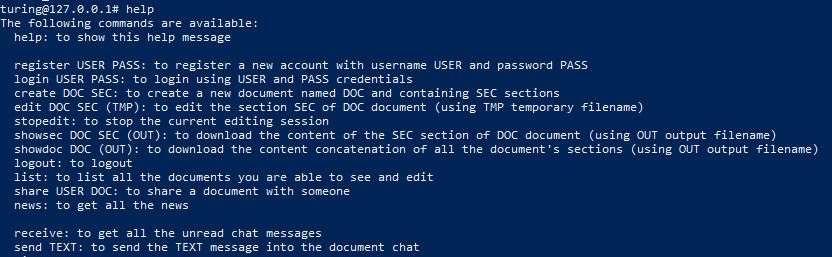
\includegraphics[width=0.8\linewidth]{assets/help_message}
\end{figure}


\section{Struttura dei Package}
I package principali, figli del root package \textit{it.azraelsec}, che fanno parte del progetto sono i seguenti:
\begin{itemize}
	\item \texttt{Chat} - Cassi che interessate nella gestione del servizio di messaggistica multicast UDP
	\item \texttt{Client} - Classi costituenti il client del sistema TURING
	\item \texttt{Document} - Classi relativi alla rappresentazione dei documenti e delle sezioni costituenti\footnote{I Documenti, infatti, sono formati in realtà da un'aggreazione di differenti Sezioni}
	\item \texttt{Notification} - Classi per la gestione delle notifiche lato client e per la loro generazione lato server
	\item \texttt{Protocol} - Classi ed interfacce atte alla gestione del protocollo di rete \textit{low-level}
	\item \texttt{Server} - Classi costituenti il server del sistema TURING, relative alla gestione del concetto di \textit{Utente} ed al ciclo di vita delle sue sessioni
\end{itemize}
\begin{figure}[h]
	\caption{UML - Package Diagram}
	\centering
	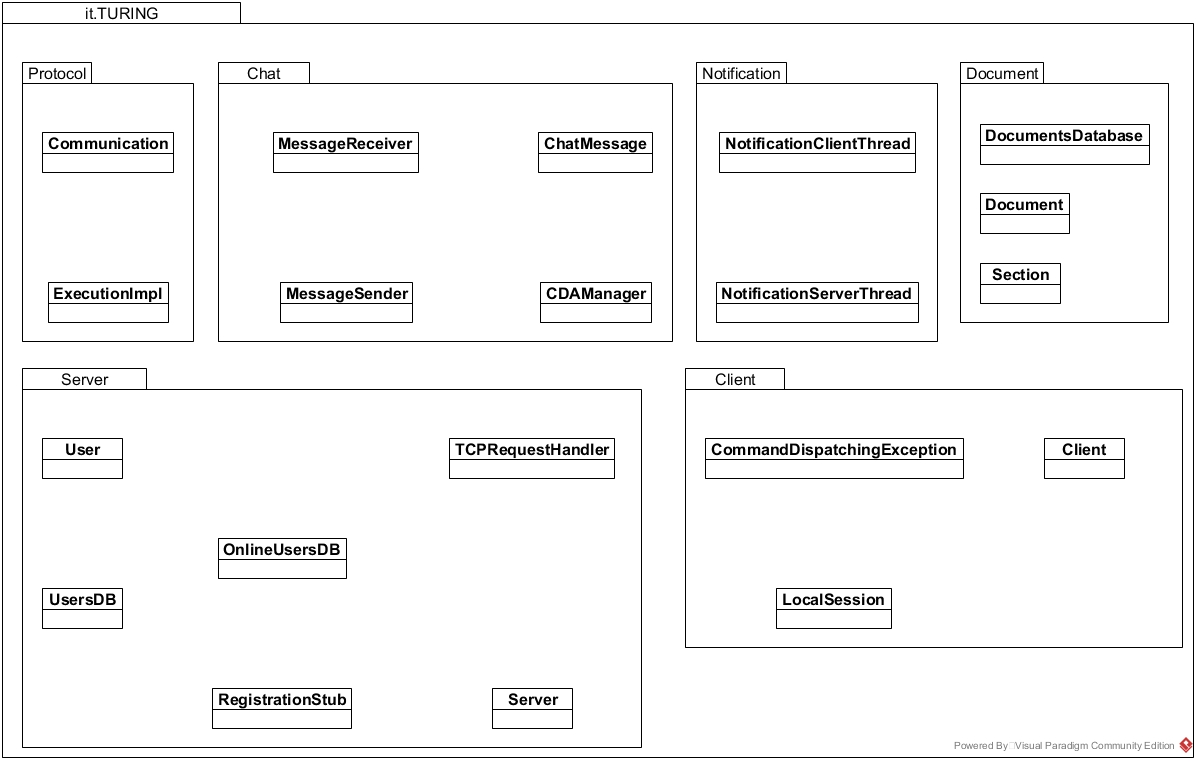
\includegraphics[width=1\linewidth]{assets/package_diagram}
\end{figure}

\pagebreak


\section{Server}


\section{Client}
Il programma client tenta di stabilire immediatamente una connessione TCP con il server: in caso di esito positivo, dà la possibilità all'utente di interagire con il sistema attraverso una riga di comando, e interrompe con esito negativo l'esecuzione in caso contrario.

A differenza del server, il client non si serve di alcuna persistenza dei dati, ma necessita in ogni caso di una directory di lavoro da sfruttare per la memorizzazione dei file che gli vengono inviati dal server per permettere la modifica delle sezioni o per la ricezione del contenuto attuale dei documenti. Il meccanismo utilizzato per la verifica dell'esistenza e validità di tale directory è identico a quello utilizzato dal server.

\paragraph{Thread Life-cycle}
Lo scambio di comandi e risultati avviene all'interno del thread principale, ma viene delegata a thread secondari la gestione delle notifiche e la ricezione dei messaggi multicast diretti al gruppo di cui il client è membro.

\begin{figure}[h]
	\caption{Client - Ciclo di vita dei Thread}
	\centering
	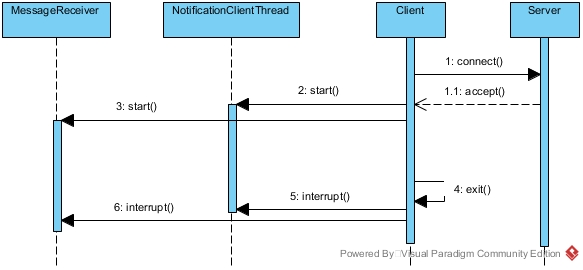
\includegraphics[scale=0.5]{assets/client/thread_activation_sequence_diagram}
\end{figure}

\newpage

\section{Protocollo di scambio}
Il protocollo utilizzato per lo scambio di messaggi è molto semplice e si basa sulla ricezione da parte del server di comandi e del successivo invio di esito dell'operazione al client. Ogni operazione, infatti, può portare all'invio da parte del server di una risposta \textbf{success} o \textbf{failure} \footnote{Si è scelto di generalizzare quanto più possibile il concetto di \textit{messaggio}, così da includervi anche quelli di risposta}.

Dunque, tutti i tipi di messaggi scambiati sono inglobati all'interno dell'enum \textbf{Commands}:
\begin{multicols}{2}
	\begin{itemize}
		\item LOGIN
		\item LOGOUT
		\item CREATE
		\item EDIT
		\item EDIT\_END
		\item SHOW\_SECTION
		\item SHOW\_DOCUMENT
	\end{itemize}
	\begin{itemize}
		\item LIST
		\item SHARE
		\item SUCCESS
		\item FAILURE
		\item NEW\_NOTIFICATIONS
		\item EXIT
	\end{itemize}
\end{multicols}
Per ognuno di questi, viene definito un array di tipi, così da dare la possibilità al client di controllare che il tipo di dato degli argomenti inviati sia corretto e per permettere al server di inferire l'ordine ed il tipo di \textit{receive()} da effettuare per ricostruire i dati inviati. Nella sezione \ref{rappresentazione_dei_dati} verrà chiarito meglio in che modo questi vengano scambiati a partire dai loro tipi.

Il protocollo prevede anche delle procedure per lo scambio di stream di dati, utili per l'invio e ricezione da parte del server del contenuto dei file rappresentanti le sezioni dei documenti o la loro concatenazione\footnote{Infatti, durante l'esecuzione del comando \textbf{SHOW\_DOCUMENT}, il server si serve della concatenazione di più stream di file per crearne uno unico da poter inviare al client, sfruttando la funzione appena descritta} .
L'invio di stream dev'essere \underline{necessariamente} preceduto da un normale invio di esito da parte del server per evitare la rottura del protocollo.

\paragraph{Approccio Funzionale}
L'approccio utilizzato nella stesura del codice relativo all'implementazione del protocollo è fortemente funzionale e segue le tecniche più moderne, coinvolgendo la definizione di appositi handler chiamati in base all'esito delle operazioni. Il listing \ref{lst:functional} è un chiaro esempio di come la programmazione funzionale venga impiegata nell'utilizzo del protocollo.

\begin{lstlisting}[language=java, caption="Frammento in cui si evidenzia l'approccio funzionale del protocollo", label={lst:functional}, float]
private void documentsList() {
	if (session != null)
		Communication.send(
			clientOutputStream,
			clientInputStream,
			System.out::println, System.err::println,
			Commands.LIST);
	else System.err.println("You're not logged in");
}
\end{lstlisting}

\subsection{Rappresentazione dei dati}\label{rappresentazione_dei_dati}
Vengono utilizzati degli oggetti di tipo \textbf{DataInputStream} e \textbf{DataOutputStream} rispettivamente per la ricezione e l'invio dei dati sul socket, per riuscire ad inviarne la corretta rappresentazione in byte\footnote{Molto utile per l'invio corretto di interi, per esempio, evitando di dover effettuare interpretazione di testo contenente la loro rappresentazione}. Se per gli interi questo approccio risulta sufficiente ad assicurarne correttamente lo scambio, per le stringhe si è dovuto far affidamento all'invio di una informazione addizionale: il numero di byte che le compongono. Infatti, ogni volta che si presenta la necessità di inviare una stringa, si procede prima alla \textit{send()} del numero di byte che la compongono e successivamente a quella dell'array dei dati. In questo modo, utilizzando l'approccio contrario, è possibile sapere di preciso quanti byte appartenenti alla stringa da ricevere prelevare dal buffer.

\begin{figure}[h]
	\caption{Schema di rappresentazione delle stringhe}
	\centering
	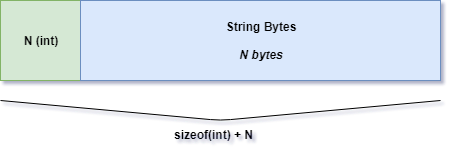
\includegraphics[scale=0.6]{assets/string_representation.png}
\end{figure}

\subsection{Sistema di notifiche}
Il sistema di notifiche è un esempio 

\end{document}

